% !TEX root = ../main.tex
\chapter{Introduction}
\label{chapter:Introduction}


\section{Motivation}

\begin{description}
	\item[SeisSol]
    Simulates earthquakes, specifically, dynamic rupture processes and seismic wave propagation over an unstructured tetrahedral mesh. 

    \item[ADER-DG]
    A numerical method which uses Discontinuous Galerkin discretization in space and ADER discretization in time. It avoids a global system matrix, using local element matrix operations instead.

    \item[Small Sparse Matrix Multiplications]
    The compute kernels resemble the operation shown below, applied recursively. Different sparsity patterns are used, but they are all known at compile time.
\end{description}

\begin{figure}
  \centering
  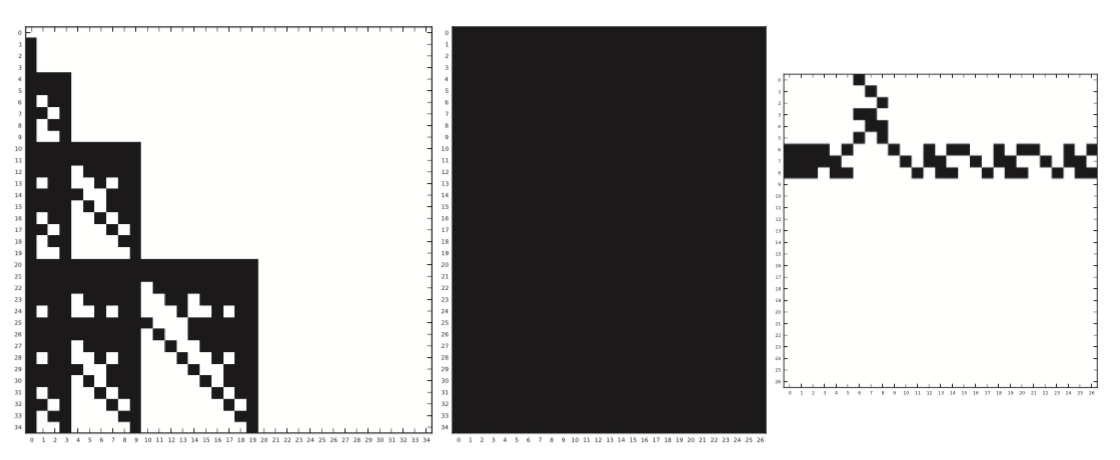
\includegraphics[height=3cm]{images/seissol_visc.png}
  \caption{Common sparsity patterns in SeisSol}
  \label{fig:seissol_star}
\end{figure}

\section{Hardware Constraints}

Although the motivation is straightforward, it is growing increasingly difficult to implement in practice because it is working against current trends in computer architecture. An increasing number of the top500 computers are using GPUs or Xeon Phis. This trend is likely to continue because it allows greater parallelism at a lower energy cost. It was desired to run the code on LRZ's CoolMUC3 cluster, which uses Knights Landing.

Knights Landing (KNL) is the second-generation Intel Xeon Phi, a manycore processor. Unlike its predecessor, Knights Corner, KNL is a host processor rather than a coprocessor, which means that it can run the entire x86-64 instruction set, albeit with a performance penalty for some operations. Each processor contains \~64 cores with 4 hyperthreads per core, resulting in 256 logical CPUs. The instruction-level parallelism is similarly impressive, being the first processor to implement the AVX-512 instruction set extensions. These provide 32 vector registers, each of which holds 64 bytes, allowing 8 double-precision floating point numbers to be operated on simultaneously in each vector processing unit (VPU). Instruction-level performance is further enhanced by a more featureful fused-multiply-add (FMA) instruction, which performs $c := c + a*b$ in a single cycle, optionally including a broadcast and a mask. Thus the theoretical peak performance of a single core is given as:

\[2 \frac{VPUs}{core} \times  = 3 {double TFlop}{sec}\]

This peak performance is in practice merely an upper bound, as it assumes a steady-state throughput of 2 FMAs per cycle. The only algorithms which performs anywhere near this bound are dense matrix multiplication and (to a lesser extent) LU and Cholesky factorization. If the algorithm is not able to be vectorized at all, the attainable performance drops by a factor of 8, and if it cannot use the FMA instructions, it drops by a further factor of 2. The standard sparse multiplication algorithms rely heavily on. 

\begin{itemize}
    \item Scalar operations limited to 1/8 peak performance
    \item Bottleneck with vector stores: 64B/cycle
    \item Bottleneck with instruction cache, decoder: min(16B/cycle, 2 instructions)
    \item \textbf{Out-of-order execution pipeline can only issue 2 instructions per cycle}
\end{itemize}

\section{Previous approaches}

  Standard compressed-sparse-column multiplication
    \begin{itemize}
      \item[$+$] Generality.
      \item[$+$] Algorithm uses a (small) constant number of instructions.
      \item[$-$] Index lookups require indirect memory access, causing lots of problems for the execution pipeline.
      \item[$-$] $sparse \times sparse$ is fundamentally scalar. (However, BSR can be vectorized.)
      \item[$-$] Disregards the fact that the sparsity pattern is known at compile time.
    \end{itemize}

  Sparsity pattern unrolled into instruction stream
    \begin{itemize}
    \item[$+$] Index lookups removed completely
    \item[$+$] $dense \times sparse$ case can be vectorized perfectly 
    \item[$-$] Generates one FMA instruction for every nonzero
    \item[$-$] (Implementation) Memory access pattern is suboptimal on KNL
    \item[$-$] (Implementation) Intel compiler struggles to generate efficient assembly
    \end{itemize}

  Current approach: Dense matrix multiplication via libxsmm
    \begin{itemize}
    \item[$+$] Memory access patterns and register blockings optimized for KNL
    \item[$+$] (Implementation) Code generator emits assembly directly 
    \item[$-$] Filling in zero entries wastes both flops and memory bandwidth
    \end{itemize}


  \section{Goals and approach}
  My approach
    \begin{itemize}
    \item The three existing algorithms each encounter different constraints and bottlenecks.
    \item Think of them as poles in a design space. Explore algorithms which combine their features in order to finesse around the bottlenecks.
    \item Speed up applications such as SeisSol, or demonstrate why it can't be done.
    \item Create a code generator which autotunes a sparse gemm algorithm for a reasonably arbitrary problem.
    \end{itemize}

 Goals
   - Explore the parameter space of different families of algorithms:
     + dense-sparse csc, tiledcsc, blockcsc
     + sparse-dense breuer, blended, shifted-load, scalar, gather-scatter

   - Independent variables include matrix size, overall sparsity, sparsity patterns, block size, register usage, loop unroll depth, instruction reordering

   - Identify bottlenecks and understand how they constrain the regions of parameter space in which they are useful

   
    \section{Remainder of paper}


\comment{You can also put comments in the margins for you or your advisor}

\begin{equation}
	\pi = \mathrm{e}^{i\cdot\phi}
	\label{eq:equation1}
\end{equation}

\begin{listing}
	%the language syntax can be declared here.
	\begin{minted}{python} 
	import numpy as np
	\end{minted}
  \caption{My nice listing}
  \label{lst:nice_listing}
\end{listing}
